\label{type_e001}
We mentioned in chapter \ref{symtab_e002} that
frontend inserts a variable in program text into symbol table
for the declaration. One of attributes of a variable is it's type.
And we also mentioned in chapter \ref{_3ac_e001} that
frontend must generates every 3 address code of which operands make
sense, especially its type.

In this chapter, we'll think about the way to express types.
Bibliography \cite{doragon} chapter 6 suggests that we
use {\em type expression} for this purpose. For example,
\begin{verbatim}
void (*signal(int, void (*)(int)))(int);
\end{verbatim}
{\em Type expression} for this declaration becomes figure
\ref{type_e006}.

\hspace{0.5cm}
\begin{figure}[htbp]
\begin{center}
\begin{latexonly}
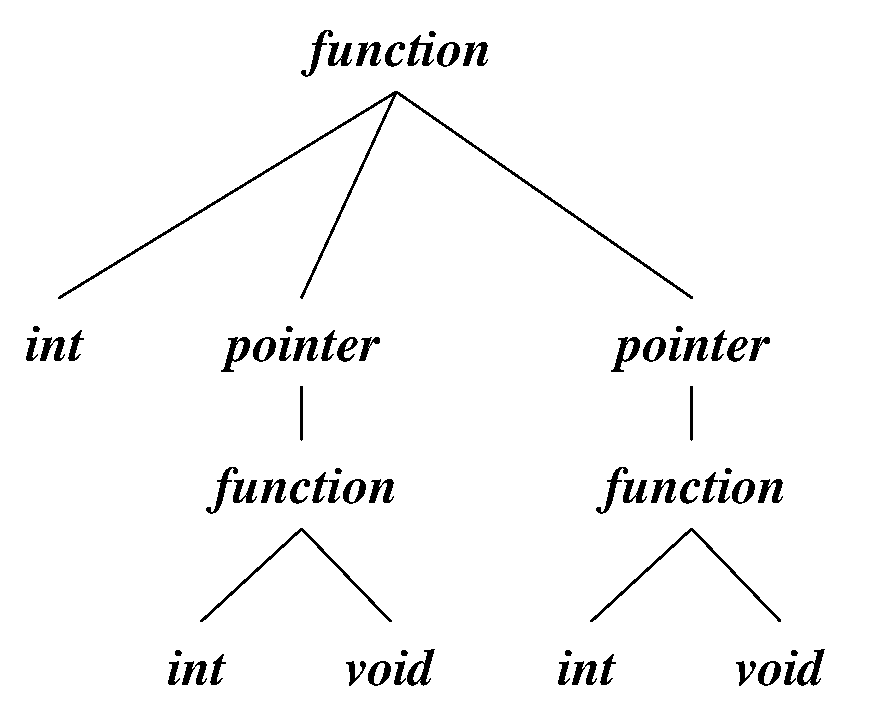
\includegraphics[width=0.5\linewidth,height=0.5\linewidth]{type_expr.eps}
\end{latexonly}
\begin{htmlonly}
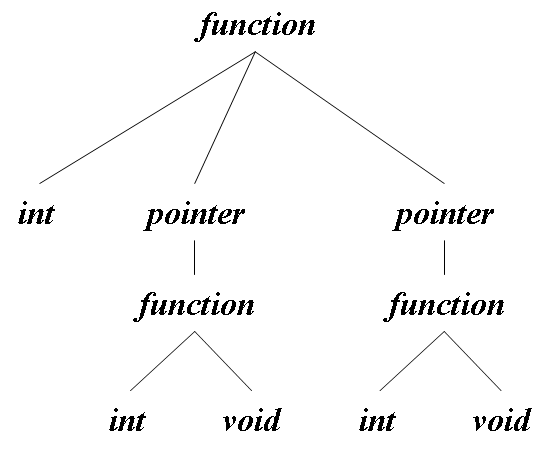
\includegraphics{type_expr.png}
\end{htmlonly}
\caption{{\em Type expression} of {\tt{signal}}}
\label{type_e006}
\end{center}
\end{figure}

That is, type can be expressed by tree.

Bibliography \cite{doragon} chapter 6 says that
{\em type expression} should be expressed by {\em dag}
(direct acyclic graph) not normal tree, because
compiler can judge equivalency of type easily. Frontend of C compiler
must also judge whether type $T_1$ is {\it compatible} with
type $T_2$, so we'll use {\em dag}. Figure \ref{type_e000}
shows {\em dag} for {\tt{signal}}.

\hspace{0.5cm}
\begin{figure}[htbp]
\begin{center}
\begin{latexonly}
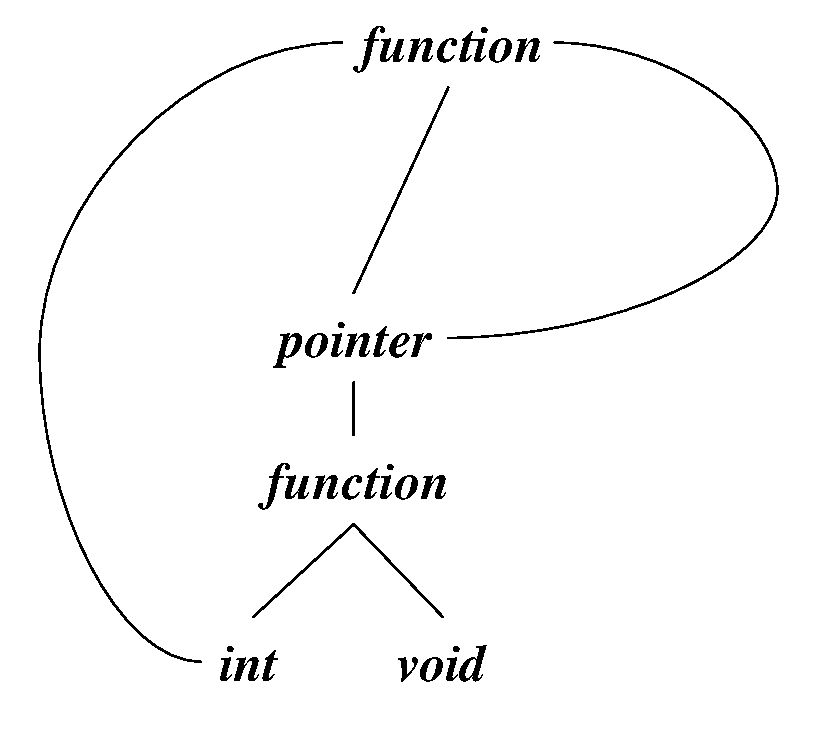
\includegraphics[width=0.5\linewidth,height=0.5\linewidth]{dag.eps}
\end{latexonly}
\begin{htmlonly}
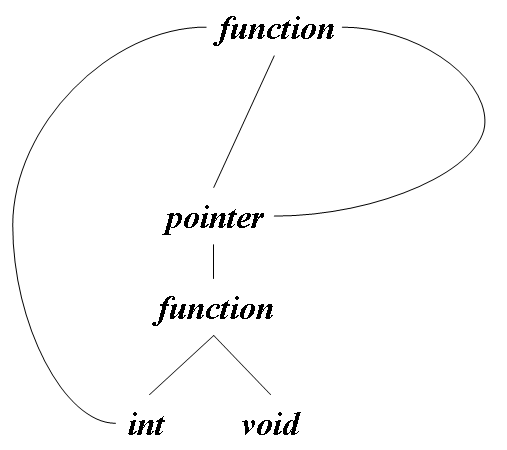
\includegraphics[width=0.3\linewidth,height=0.3\linewidth]{dag.png}
\end{htmlonly} 
\caption{{\em dag} of {\tt{signal}}}
\label{type_e000}
\end{center}
\end{figure}

Now, we'll define base class to judge {\it compatibility}.
\begin{verbatim}
class type {
public:
  ...
  virtual bool compatible(const type* that) const
  {
    return this == that->unqualified();
  }
  ...
};
\end{verbatim}
Please note that the equality of type can be judged by
comparing the address of types.
Other many virtual function for {\tt{type}} are necessary,
but in this chapter, we just think about {\it compatiblity} of type.

\section{Basic type}

Bellow table shows C language basic type and its class.

\begin{latexonly}
\vspace{0.5cm}
\end{latexonly}

\begin{tabular}{|l|l|} \hline
C language & its class \\ \hline
{\tt{void}} & {\tt{void\_type}} \\ \hline
{\tt{char}} & {\tt{char\_type}} \\  \hline
{\tt{signed char}} & {\tt{schar\_type}} \\  \hline
{\tt{unsigned char}} & {\tt{uchar\_type}} \\  \hline
{\tt{short int}} & {\tt{short\_type}} \\  \hline
{\tt{unsigned short int}} & {\tt{ushort\_type}} \\  \hline
{\tt{int}} & {\tt{int\_type}} \\ \hline
{\tt{unsigned int}} & {\tt{uint\_type}} \\  \hline
{\tt{long int}} & {\tt{long\_type}} \\ \hline
{\tt{unsigned long int}} & {\tt{ulong\_type}} \\ \hline
{\tt{long long int}} & {\tt{long\_long\_type}} \\ \hline
{\tt{unsigned long long int}} & {\tt{ulong\_long\_type}} \\ \hline
{\tt{float}} & {\tt{float\_type}} \\ \hline
{\tt{double}} & {\tt{double\_type}} \\ \hline
{\tt{long double}} & {\tt{long\_double\_type}} \\ \hline
\end{tabular}

\begin{latexonly}
\vspace{0.5cm}
\end{latexonly}

For example, {\tt{int\_type}} is defined like bellow.
\begin{verbatim}
class int_type : public type {
  static int_type obj;  // Only object
  int_type(){}          // private constructor
public:
  static const int_type* create(){ return &obj; }
};
\end{verbatim}

\section{Pointer}
\label{type_e003}
Pointer can be defined like bellow.
\begin{verbatim}
class pointer_type : public type {
  const type* m_T;  // referenced type
  pointer_type(const type* T) : m_T(T) {}
  typedef map<const type*, const pointer_type*> table_t;
  static table_t table;
public:
  static const pointer_type* create(const type* T)
  {
    table_t::const_iterator p = table.find(T);
    if (p != table.end())
      return p->second;  // already exists, return it.
    else
      return table[T] = new pointer_type(T);
  }
  bool compatible(const type* T) const
  {
    typedef const pointer_type PT;
    PT* that = dyanmic_cast<PT*>(T);
    if (!that)
      return false;
    return this->m_T->compatible(that->m_T);
  }
  ...
};
\end{verbatim}

\section{Qualifier}
\label{type_e002}
There are 3 qualifiers {\tt{const}}, {\tt{volatile}} and {\tt{restrict}}
in C language.
For example, {\tt{const}} can be expressed like bellow.
\begin{verbatim}
class const_type : public type {
  const type* m_T;  // qualified type
  const_type(const type* T) : m_T(T) {}
  static map<const type*, const const_type*> table;
public:
  // Return type is not const const_type*. It's const type*.
  static const type* create(const type* T);

  // Same with pointer_type::compatible
  bool compatible(const type* T) const;
  ...
};
\end{verbatim}
Someone may want to implement \tt{const\_type::create}
like {\tt{pointer\_type::create}}. But see bellow example:
\begin{verbatim}
typedef const int CI;     // const_type(int_type)
typedef volatile int VI;  // volatile_type(int_type)
volatile CI vci;  // volatile_type(const_type(int_type))
const VI cvi; // Not const_type(volatile_type(int_type))
              // Make it volatile_type(const_type(int_type))
const CI cci;  // Not cosnst_type(const_type(int_type))
               // Make it same with type of CI
\end{verbatim}
This example illustrates it's necessary to make more effort
to implement \tt{const\_type::create}. Other implementation
may chose a class which expresses all qualifier. It's necessary
to use same type object to express same type. If not,
{\it dag} implementation should be reviewed.

\section{Array}

Array has its element type and dimension, so can be defined like bellow.

\begin{verbatim}
class array_type : public type {
  const type* m_T;  // element type
  int m_dim;        // dimension
  array_type(const type* T, int dim) : m_T(T), m_dim(dim) {}
  ...
public:
  bool compatible(const type* T) const
  {
    typedef const array_type AT;
    AT* that = dynamic_cast<AT*>(T);
    if (!that)
      return false;
    if (!this->m_T->compatible(that->m_T))
      return false;
    if ( this->m_dim && that->m_dim )
      return this->m_dim == that->m_dim;
    return true;  // one is, or both are incomplete array.
  }
  ...
};
\end{verbatim}
See bellow declarations:
\begin{verbatim}
int a[10];
...
extern int a[];
\end{verbatim}
In 1st declaration, type of \tt{a} is
\tt{array\_type(int\_type, 10)} and 2nd declaration,
\tt{array\_type(int\_type, 0)}. 2 types are not
same, but are compatible, so 2nd declaration is
not error. Frontend may register the type of \tt{a}
as \tt{array\_type(int\_type, 10)} not
\tt{array\_type(int\_type, 0)}.

To digress a little, array cannot or should not be qualified.
For the declarations
\begin{verbatim}
typedef int A[10][20];
const A a;
\end{verbatim}
frontend should constitute {\em type expression} of {\t{a}}
like figure \ref{type007}. Figure \ref{type008} is not fine.
\begin{figure}[htbp]
\begin{center}
\begin{latexonly}
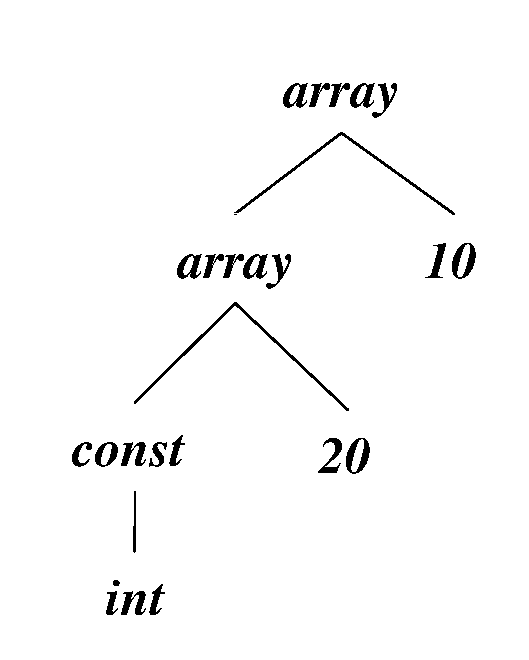
\includegraphics[width=0.4\linewidth,height=0.5\linewidth]{correct_array.eps}
\end{latexonly}
\begin{htmlonly}
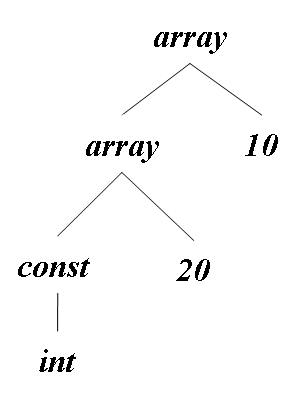
\includegraphics{correct_array.png}
\end{htmlonly}
\caption{correct {\em type expression} of {\tt{a}}}
\label{type007}
\end{center}
\end{figure}
\begin{figure}[htbp]
\begin{center}
\begin{latexonly}
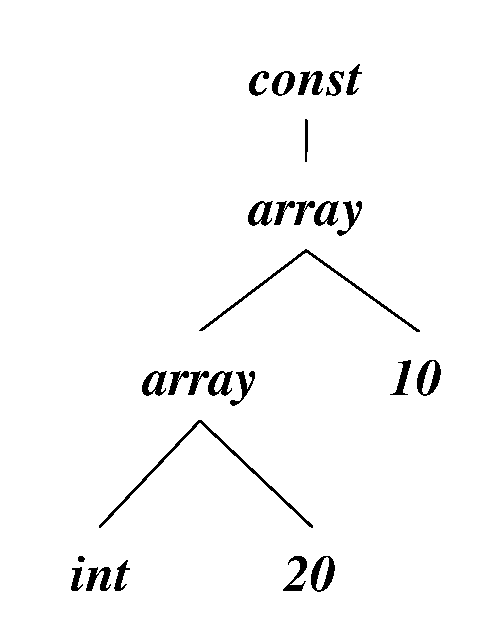
\includegraphics[width=0.4\linewidth,height=0.5\linewidth]{incorrect_array.eps}
\end{latexonly}
\begin{htmlonly}
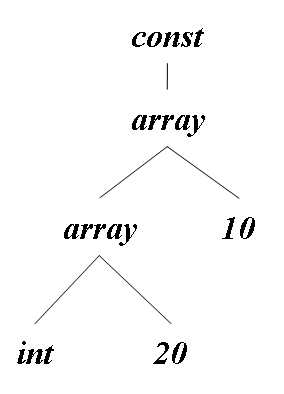
\includegraphics{incorrect_array.png}
\end{htmlonly}
\caption{incorrect {\em type expression} of {\tt{a}}}
\label{type008}
\end{center}
\end{figure}

\section{Function}

Function can be defined like bellow.
\begin{verbatim}
class func_type : public type {
  const type* m_T;              // return type
  vector<const type*> m_param;  // parameter types
  ...
public:
  bool compatible(const type*) const;
}
\end{verbatim}

Override member function {\tt{func\_type::compatible}}
becomes a little complicated.

\begin{verbatim}
bool func_type::compatible(const type* T) const
{
  typedef const func_type FT;
  FT* that = dynamic_cast<FT*>(T);
  if (!that)
    return false;  // not function
  if (!this->m_T->compatible(that->m_T))
    return false;  // not compatible return type
  if (this->m_param.size() != that->m_param.size()) {
    // possible old style, but here simply return false
    return false;
  }
  vector<const type*>& u = this->m_param;
  vector<const type*>& v = that->m_param;
  pair<IT,IT> p = mismatch(u.begin(),u.end(),v.begin(),::compatible);
  return p == make_pair(u.end(),v.end());
}
\end{verbatim}

\subsection{Variable arguments}
\label{type_e004}
In C language, function can take variable arguments.
We denotes class {\tt{ellipsis\_type}} to be ellipsis ( \tt{...}).
For example, the declaration in {\tt{stdio.h}},
\begin{verbatim}
extern int printf(const char* fmt, ...);
\end{verbatim}
for this declaration, frontend constructs {\em type expression}
like figure \ref{type_e009}.
\begin{figure}[htbp]
\begin{center}
\begin{latexonly}
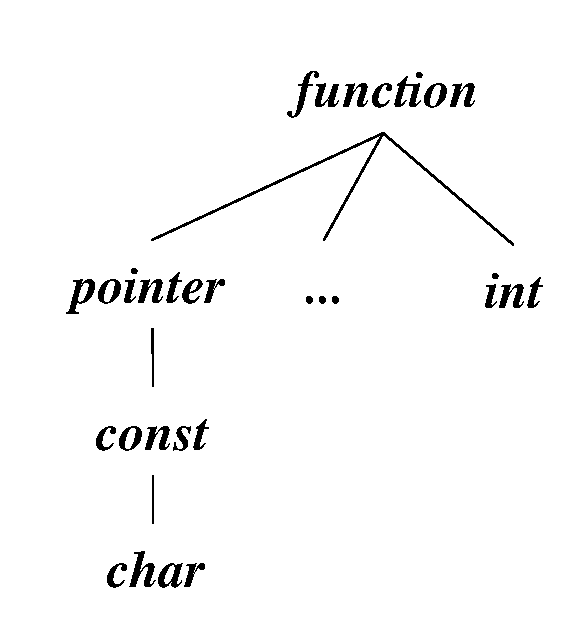
\includegraphics[width=0.5\linewidth,height=0.5\linewidth]{ellipsis_type.eps}
\end{latexonly}
\begin{htmlonly}
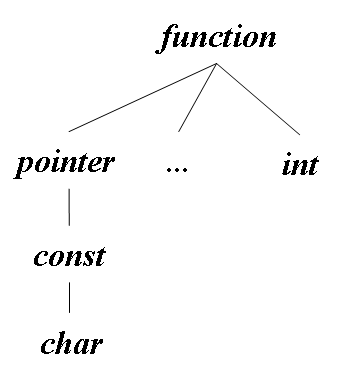
\includegraphics{ellipsis_type.png}
\end{htmlonly}
\caption{{\em type expression} of {\tt{printf}}}
\label{type_e009}
\end{center}
\end{figure}

\section{Tagged types}
\label{type_e010}
In C language, sturcture, union or enumeration is
associated with its tag. And its tag is associated
with its type, too. Here, we'll think about such types.
For example,
\begin{verbatim}
struct S { int m; } a;
void f(void)
{
  struct S { int m; } b;
  a = b; /* error */
}
\end{verbatim}
Compiler outputs error message like the assignment is applied for 
not compatible structure objects. This example shows
that structure is associated with its tag, not object layout.

\subsection{Structure, union}

Structure or union are referenced its member offset and type by name.
Not only tag and members, but also layout infomation should be
contained.

\begin{verbatim}
class record_type : public type {
  tag* m_tag;  // tag
  vector<usr*> m_member;  // member

  // layout infomation of structure or union
  map<string, pair<int, const type*> > m_layout;
  ...
public:
  bool compatible(const type* that) const
  {
    typedef const record_type RT;
    RT* that = dynamic_cast<RT*>(T);
    if (this == that)
      return true;
    typedef const const incomplete_tagged_type ITT;
    ITT* itt = dynamic_cast<ITT*>(T);
    if (!itt)
      return false;
    return m_tag == itt->get_tag();
  }
  ...
};
\end{verbatim}

\subsection{Enumeration}

Frontend must add enumeration members into symbol table, not into
its type. This is different with structure or union. 
\begin{verbatim}
class enum_type : public type {
  tag* m_tag;
  ...
public:
  // judge samely with record_type::compatible
  bool compatible(const type* T) const;
  ...
};
\end{verbatim}

\subsection{Incomplete tagged type}

It's possible to declare structure, union and enumeration without
members in C language. But please note that incomplete tagged type
is necessary for parsing or analising
complete structure, union and enumeration type.
For example,
\begin{verbatim}
struct tree {  /* add tag for struct tree into symbol table */

  struct tree* left;  /* lookup symbol table and know struct tree
                         is incomplete structure type */
  struct tree* right;
  int v;
}; /* struct tree becomes complete structure type */

enum E { /* add tag for enum E into symbol table */

   a = sizeof(enum E), /* lookup symbol table and know enum E
                          is incomplete type. This is error */
   b,
};
\end{verbatim}

Incomplete tagged type is defined like bellow.
\begin{verbatim}
class incomplete_tagged_type : public type {
  tag* m_tag;
  ...
public:
  // judge samely with record_type::compatible
  bool compatible(const type* T) const;
  ...
};
\end{verbatim}

\section{Bit field}

We don't have to search if bit field is compatible
to type $T$, because bit field is member of structure
or union. Structure or union {\it compatiblity} is
depend its tag. But it's necessary to remember
the member is bit field.

\begin{verbatim}
class bit_field_type : public type {
  int m_bit;          // number of bit
  const type* m_T;    // integer type
  ...
};
\end{verbatim}
